%!TEX root = ../notes.tex
\section{March 14, 2022}
\subsection{Elliptic Curves}
An \ul{elliptic curve} is an equation of the form
\[y^2 = x^3 + ax + b\]
It looks like this:
\begin{center}
    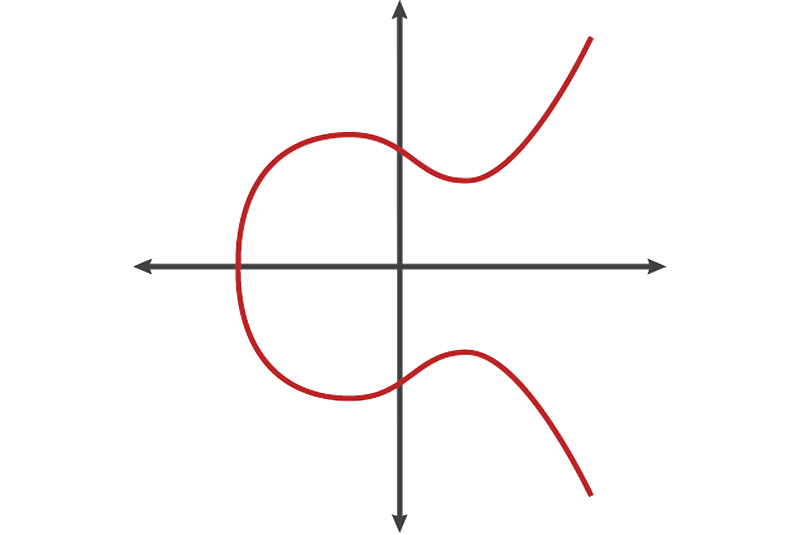
\includegraphics[width=0.6\textwidth]{images/elliptic_curve.png}
\end{center}

\emph{What's special about cubic equations?} We have a special property that every line $L$ meets $E$ in 3 points.

\emph{What happens when we have a tangential line?} We count multiplicity.

\emph{What happens when it only meets at 1 or 2 points?} We count complex roots.

\emph{What happens with vertical lines that only meet at 2 points?} We include $\cO = \text{``point at $\infty$''}$.

\emph{Where does $\cO$ come from?} It comes from the $\RR\mathbb{P}^2$ (the real projective plane) or $\CC\mathbb{P}^2$ (the complex projective plane).

Given two points $A$ and $B$, we can get a third point $C$ which is the third point on the line passing through $A$ and $B$. Taking this as a binary operation...does this give us a group?

Consider:
\begin{align*}
    A + B & = C           \\
    A + C & = B           \\
    A + A & = \cO\text{?}
\end{align*}
Maybe we can declare
\[A + B + C = \cO\]
If we call the reflection of $C$ across the $x$-axis is $D$, we have
\begin{align*}
    A + B + C   & = \cO \\
    C + D + \cO & = \cO \\
    A + B       & = D
\end{align*}
So we have that the group law is $A + B$ is the reflection of the third point $C$ across the $x$-axis.
\begin{definition}[Elliptic Curve]
    An \ul{elliptic curve} is the set of solutions to
    \[y^2 = x^3 + ax + b\]
    plus a point $\cO$ at infinity...where $a, b$ satisfy $4a^3 + 27b^2\neq 0$.
\end{definition}

Recall from high school that $ax^2 + bx + c$ gives discriminant $\Delta = b^2 - 4ac$. Taking a cubic equation $x^3 + ax + b$, the discriminant is $\Delta = -16(4a^3 + 27b^2)$. This is also saying $x^3 + ax + b$ has no repeated roots. For it to be tangent to the $x$-axis, it has to self-intersect. But every line passing through the intersection is a tangent line. Messy messy things happen:
\begin{center}
    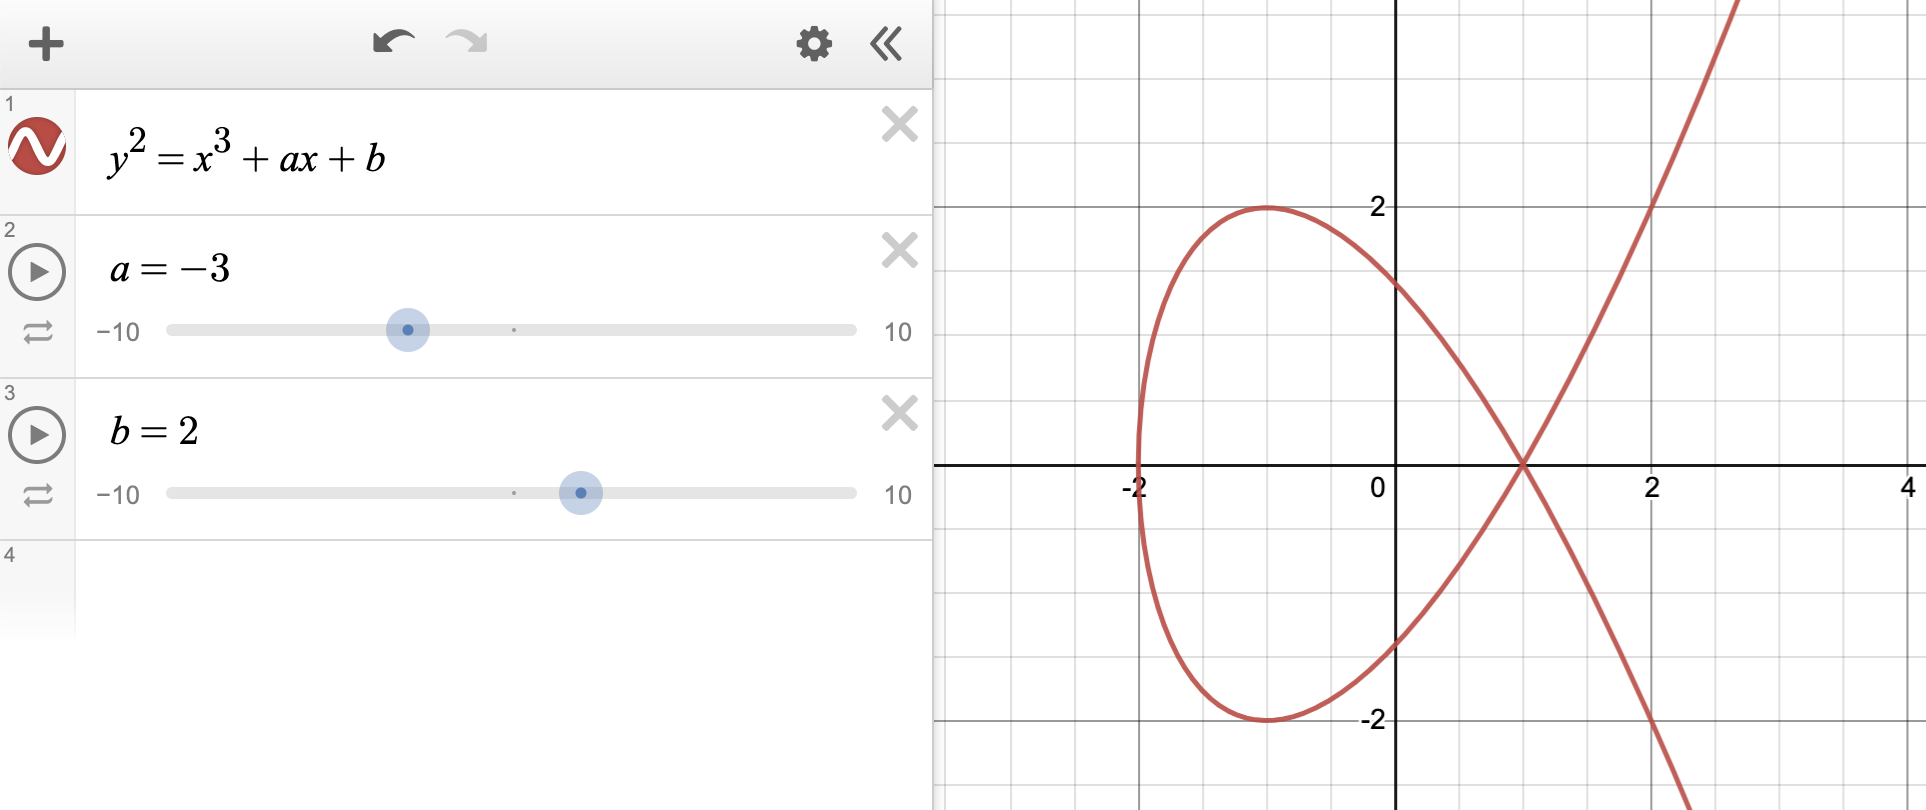
\includegraphics[width=0.8\textwidth]{images/fish.png}
\end{center}

We take the fact that an elliptic curve is a group on faith, with the group operation defined above.

\subsection{Addition on Elliptic Curves}
\begin{itemize}
    \item $P + \cO = \cO + P = P$. That is, $\cO$ is the identity.
    \item If for points $P_1 = (x_1, y_1), P_2 = (x_2, y_2)$ and $x_1 = x_2$, $y_1 = -y_2$. Then $P_1 + P_2 = \cO$.
    \item If $P_1 \neq P_2$, $\lambda = \text{Slope of $L$} = \frac{y_2-y_1}{x_2-x_1}$. So the equation of $L$ is $y-y_1 = \lambda(x-x_1)$. (We find the third point and reflect it). Will pick up here on Wednesday.
\end{itemize}